\documentclass[manuscript]{aastex}

\newcommand{\vdag}{(v)^\dagger}
\newcommand{\ie}{{\it i.e., }}
\newcommand{\eg}{{\it e.g., }}
\newcommand{\myemail}{steinkirch@gmail.com}



\begin{document}


\title{On the Calculation of the Angular Diameter \\of the Sun by Milchelson Radio Interferometry}
\author{{\bf Marina von Steinkirch} \\ (laboratory partners: A. Massari and M. von Hippel)}
\affil{State University of New York at Stony Brook \\ Department of  Physics and Astronomy  }



\begin{abstract}
We report the measurement of the angular diameter of the Sun with two complementary analysis. The observations were perfomed with  the Stony Brook radio interfometer, a compact interferometer that exploits  suitable wavelengths to resolve the magnitudes of the experiment. We measured the total power of the Sun and of a point source for different distances between the mirrors. We compare the results of the interfermeter to the simple beam pattern scan. The fringe pattern by the interferometry data was normalized and Fourier-analyzed. The peak frequencies were identified and the diameter of the Sun was inferred from two methods: (i)  by Taylor-expanding the visibility function, and (ii) by fitting the Fourier-transformed {\it sinc} visibility function. We verified a value of $\Phi^{Tay}_{sun} = 37.43' \pm 5.33' $ and $\Phi^{Fit}_{sun}= 32.77' \pm 5.28'$, respectively. Both values are compatibles to the actual  value in the literature,  $\Phi^{Actual}_{sun}= 31.1' \pm 0.6'$.

\end{abstract}
\keywords{Radio Interferometry: general --- Radio Interferometry: Michelson, Sun}





\section{Introduction}
% a contextual description of the goals of experiment

In 1921, Michelson and Peace developed the concept of {\it astronomy interferometry} \cite{michel}, measuring the {\it angular diameter} of one the brightness star in the sky, {\it Betelgeuse}, with an {\it optical telescope}. Nowadays,  Michelson and Peace techniques have broad applications in astronomy to measure stellar diameters \cite{sbu}.

{\it Optical} (wavelength ranges of 390 to 750 nanometers) or {\it Radio interference} (wavelength range of hundreds of meters to millimeters) \cite{wiki} can be achieved by superimposing signals from more than one telescope, yielding superior {\it resolutions} than that offered by the telescope alone \cite{brand}. This is due the fact that the orders of magnitude of the wavelengths in the radio electromagnetic spectra are scalables to the {\it baselines distances}. Interferometry is a powerful tool in radio astronomy. 

A {\it radio interferometer} measuring an extensive source such as the Sun will show a proportional relation of the dimensions of the experiment (\ie measurable baseline lengths), to the radio wavelength detected, and  to the {\it sizes of fringe}, in the resulting power spectra. In addition, precise values for the baseline lengths can be inferred by observing the power spectra of a point source (\eg an artificial geostationary satellite).

In our experiment, we make use of a two-mirrors  radio interferometer, assembled in the Stony Brook University\cite{sbu}, to measure the angular diameter of the Sun, $\Phi_{sun}$. We show that the Sun is roughly resolved when viewed in {\it single-dish mode}, but it is well resolved when {\it observed interferometrically}. 
\bigskip


\subsection{The Geometry of Radio Interferometry}

The principle of {\it superposition of waves}, figure \ref{int}, states that when two or more waves are incident on the same point, the {\it total displacement} at that point is equal to the {\it vector sum of the displacements of the individual waves}. If a crest of a wave meets a crest of another wave of the same frequency at the same point, the {\it magnitude of the displacement} is the {\it sum of the individual magnitudes}, yielding a {\it constructive interference}. If a crest of one wave meets a trough of another wave, the magnitude of the displacements equals the difference in the individual magnitudes, yielding a {\it  destructive interference} \cite{brand}.

\begin{figure}[htb]
\begin{center}
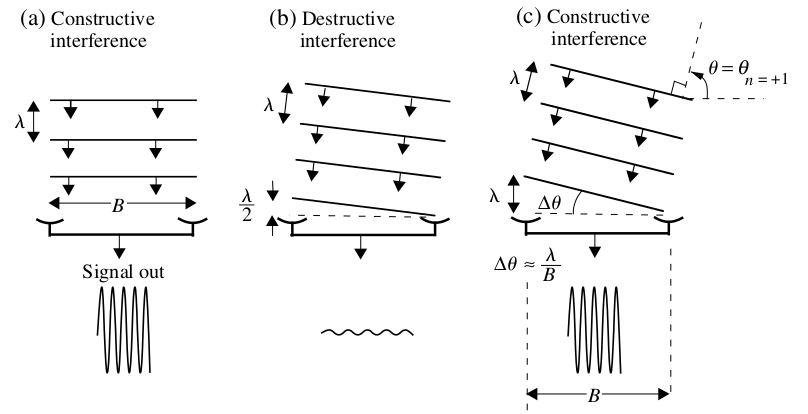
\includegraphics[scale=0.55]{figs/inter.png}
\caption{Interference between two plane wave from a distance source at different angles, from \cite{brand}. The signals are vectorially added, constructively (a), (c), and destructively  (b). }
 \end{center}
\label{int}
\end{figure}



An interferometer will detect and vectorially add signals from two different positions, figure \ref{fig:t}-a. The signal arrives on the two {\it mirrors}, being then mixed in the {\it antenna receiver}. The separation between the two positions (mirrors) is named {\it baseline length}, $B$.

\begin{figure}[htb]
\begin{center}

 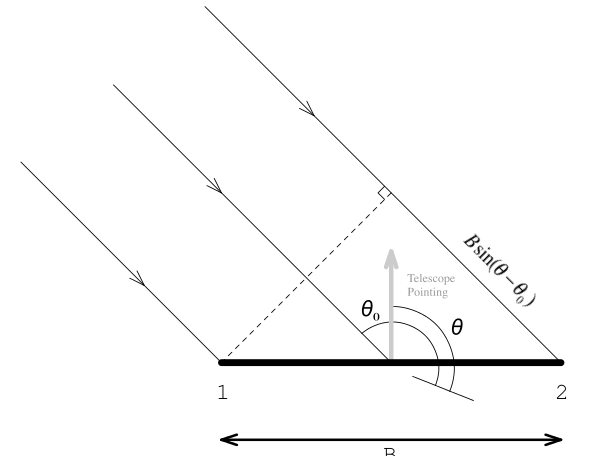
\includegraphics[scale=0.45]{figs/time.png}  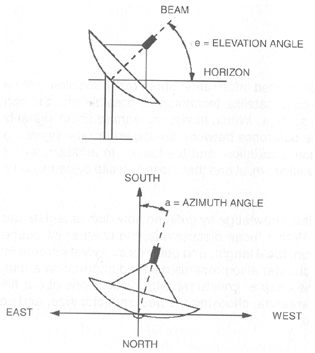
\includegraphics[scale=0.81]{figs/ele.jpg}
\caption{(left)  a -  Signal detection on two mirrors on a radio telescope separated by a baseline length $B$, from \cite{sbu}. (right) b - Elevation and azimuth angles in the dish.}
\label{fig:t}
 
\end{center}
\end{figure}


From an arbitrary origin, we define the horizontal variable angle of the telescope pointing, $\theta$, and the fixed horizontal angle coordinates of the object in the sky, $\theta_0$, as in figure \ref{fig:t}. The angle $\theta_0$ will be later related to the actual azimuth, $A$, of the object. It will be also useful to calculate the {\it declination}, $\delta$ of the object (equatorial coordinates), that can obtained from the {\it elevation}, $E$, the {\it azimuth}, and the geographical latitude $\phi$ (horizontal coordinates)\cite{wiki},
\begin{equation}
\sin \delta = \sin \phi \cdot \sin E + \cos \phi \cdot \cos E \cdot \cos A.
\label{dec}
\end{equation}



The signal wavefronts arrive at the telescope in phases because one of the sources is overhead. The {\it time delay}, $\tau$, of the signal at the position 2 (figure \ref{fig:t}-a), is related to difference between these two angles, the baseline length $B$, and the electromagnetic radiation speed, {\it c},
\begin{equation}
\tau = \frac{B \sin(\theta - \theta_0)}{c} \approx \frac{B(\theta - \theta_0)}{c},
\label{t}
\end{equation}
where we use the fact that $\theta-\theta_0\ll1$, such that the Taylor-expansion for small-angle approximation allows $    \sin \theta \approx \theta $.

\bigskip

\subsection{The Physics of Radio Interferometry}

Electromagnetic radiation can be written in terms of their perpendicular {\it electric fields, E}, and {\it magnetic fields, B}, where the last can be simply derived from the first with the {\it Maxwell Equations} \cite{jackson}.

The radio signal is electromagnetic radiation. At the frequency $\nu$, its time-sinusoidal amplitude arriving at position 1 (figure \ref{fig:t}-a) can be described as a plane wave with the  electric field  amplitude \cite{sbu},
$$\mathbf E_1(t) = \mathbf E(\theta_0)   \cos [2\pi \nu t] .$$

The signal arriving at position 2 at that same time has traveled $B \sin(\theta - \theta_0)$ more than $E_1(t)$, and its electric field amplitude  is
$$\mathbf E_2(t) =  \mathbf E(\theta_0)  \cos [2\pi \nu (t-\tau)] .$$



In the  interferometer receiver, the two signals are vectorially added,
$$
\mathbf E_{tot}(t) =  \mathbf   E_1(t) + \mathbf E_2(t),
$$
 and the receiver detects the {\it total power} of the signal, $P(t)$.  The radio frequency, $\nu$, is large compared to a data sampling rate of the receiver, and the total power detected  is {\it time averaged} (or integrated) \cite{sbu} \cite {brand} \cite{jackson},
\begin{eqnarray}
P(t) &=& \langle\mathbf E_{tot}(t)^2 \rangle, \nonumber \\
& =&   E^2(\theta_0) [1+ \cos (2\pi \nu \tau)],  \nonumber \\ 
P(\theta)&=& E^2(\theta_0) [1+ \cos (2\pi B_{\lambda} (\theta - \theta_0))],
\label{p}
\end{eqnarray}
where 
$B_{\lambda} \equiv B/\lambda,$ 
is the {\it normalized baseline length} to the wavelength $\lambda = c/\nu$ and we have applied the results from equation (\ref{t}).

Considering that the object has an extension in the sky,  we can rewrite equation (\ref{p}) as a continuum total power law,
\begin{eqnarray}
P(\theta) = \int \varepsilon (\theta_0) d\theta_0 \Bigg [1+ \cos \Big (2\pi B_{\lambda} (\theta - \theta_0)\Big)\Bigg ].
\label{p22}
\end{eqnarray}

An astronomical object can have any kind of structure, this will result on many kinds of the {\it energy density distribution},  $\varepsilon(\theta_0)$. The telescope interferometer receiver will measure the  sinusoidal power intensity response of the object given by equation (\ref{p22}), where $\theta$ are the fringes pattern due the interferometry. This quantity will be directly related to the {\it Fourier transformation} of the energy density distribution of the object.

\bigskip



\subsection{Obtaining the Baseline Lengths from a Point Source }



For a punctual source (artificial geostationary satellite), the energy density varying  on $\theta_0$ (as we sweep the telescope)  is a $\delta$-function at the position of the object:
\begin{eqnarray}
 \varepsilon_{sat} (\theta_0) = \varepsilon_0 \delta (\theta_0). 
\label{del}
\end{eqnarray}

An expect profile of the total power (amplitude squared) of a point source measured interferometrically can be seen in the figure \ref{bas}. The pattern of this figure can be thought as resolved  as a serie of point sources, slightly displaced, where the interference and the peaks and valleys shrink towards the central value of one. 


We insert equation (\ref{del}) into (\ref{p22}) and integrate. As we have mentioned in the beginning of this session,  measurements of a point source yields the accurate measurement of  baseline lengths. The total power is zero in the fringe's minimums (destructive interference, as shown in the figure \ref{int}), becomes
\begin{eqnarray}
P_{sat}(\theta) = \varepsilon_0  \Bigg [1+ \cos \Big (2\pi B_{\lambda} (\theta - \theta_0) \Big ) \Bigg] \equiv 0,
\label{p223}
\end{eqnarray}
meaning
\begin{eqnarray}
2\pi B_{\lambda} (\theta - \theta_0) & =& (2n+1) \pi  \nonumber \\
B_{\lambda} (\theta - \theta_0) & =& \frac{2n+1}{2}. \nonumber
\end{eqnarray}

Therefore, the separation between adjacent null positions (\ie the {\it angular size of the component} we are measuring) gives the value of the baseline lengths,
\begin{eqnarray}
B_{\lambda} \Delta \theta_{12} &=& \frac{2(n_1 - n_2)}{2},\nonumber \\
B^{\Delta \theta}_{\lambda} &\approx& \frac{1}{\Delta \theta}.
\end{eqnarray}
(as we can observe, again in the figure  \ref{bas}). We say it is an approximate value because the rotation of the earth plays a role here, it continuously reorients the telescope, causing the directions of the constructive/destructive interference to scan across the radio source. For instance, the earth rotates $0.5^o$ each every 2 minutes.  This oscillation/modulation should be at a much lower frequency than the radio frequency \cite{brand}.

\begin{figure}[htb]
\centering
 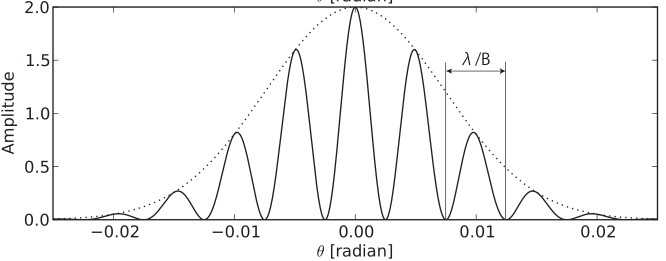
\includegraphics[scale=0.55]{figs/bas.png}
\caption{Example plot of total power as function of telescope pointing, $\theta$ for a point source such as the satellite, from \cite{sbu}. }
\label{bas}
\end{figure}


In addition, with the  actual  declination of the object, $\delta$, from equation (\ref{dec}), the fringe $\Delta \theta$ is the {\it Fourier transform} of the fringe period $\Delta t$.  Considering the angular frequency of earth rotation as $\omega = 15^o / h$, we can also obtain the baseline lengths writing 
\begin{equation}
  B^{\Delta t}_{\lambda} = \frac{1}{\cos(\delta) \sin(\omega \Delta t)}.
\label{BB}
\end{equation}

In the rest of this session, we shall write $B_{\lambda}$  for simplicity.




\bigskip

\subsection{Calculating the Angular Diameter of the Sun} \label{visb}


We can rewrite the total power given by equation (\ref{p22}),
$$ P_{sun}(\theta) = \int \varepsilon (\theta_0) d\theta_0 + \int \varepsilon (\theta_0) \cos (2\pi B_{\lambda} (\theta - \theta_0)) d\theta_0.$$

This is the the Fourier transformation of the object's energy density distribution and we can prove it rewriting the above equation in the same fashion as in \cite{sbu}:
$$P_{sun}(\theta) = S_{sun} [1+V(\theta,B_{\lambda})],$$
where
$$ S_{sun} = \int \varepsilon (\theta_0) d\theta_0,$$
is the full spectra of the Sun (obtained as a single dish rather than as interferometer), and
\begin{eqnarray}
V(\theta, B_{\lambda})&=& \frac{1}{S_{sun}} \int \varepsilon (\theta_0) \cos [2\pi B_{\lambda} (\theta-\theta_0)] d\theta_0 ,\nonumber \\
&=& V_{sun} (B_{\lambda}) \cos [2\pi B_{\lambda} \theta],
\end{eqnarray}
 where we gauge the {\it zero-phase position} of the coordinates to eliminate a phase. $V_{sun}$ is the visibility function of the Sun (an amplitude of the Fourier transform a baseline length $B_{\lambda}$),
\begin{equation}
V_{sun}(B_{\lambda}) = \frac{1}{S_{sun}} \int \varepsilon (\theta_0) e^{-i2\pi B_{\lambda} \theta_0}d\theta_0.
\end{equation}

We can compare this to the observed total power law,
$$P_{sun}(\theta) = S_{sun} \Big [1 + V_0(B_{\lambda}) \cos [2\pi B_{\lambda} (\theta - \Delta \theta)]\Big].$$

\bigskip

To extract the power function from an astronomical source, $P_{sun}(\theta)$, we sweep the object by changing the direction of the telescope pointing, $\theta$. We see a  sinusoidal curve plus an {\it offset} proportional to  $\theta$, as shown in the figure \ref{psun}, together with maximum and minimum values for the total power function.



\begin{figure}[htb]
\centering
 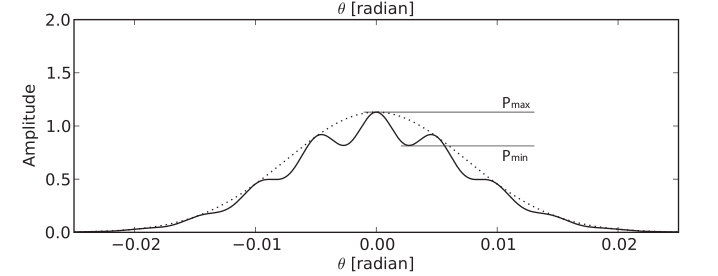
\includegraphics[scale=0.55]{figs/psun.png}
\caption{Example plot of total power as function of telescope pointing, $\theta$ for a extended source, such as the Sun, from \cite{sbu}. }
\label{psun}
\end{figure}

It is straightforward to rewrite out results in terms of $P_{max}$ and $P_{min}$,
\begin{equation}
P_{max} = S_{sun} [1 + V_{sun}(B_{\lambda})], 
\end{equation}
\begin{equation}
 P_{min} = S_{sun }[1-V_{sun}(B_{\lambda})].
\end{equation}

The {\it visibility function}  is then
\begin{eqnarray}
V_{sun}(B_{\lambda}) &=& \frac{P_{max} - P_{min}}{P_{max} + P_{min}}.
\label{vis}
\end{eqnarray}
which is a {\it sinc} function in term of  the baseline lengths,
\begin{eqnarray}
V_{sun}(B_{\lambda}) &=& \frac{\sin  ( \pi   B_{\lambda} \Phi_{sun}  )}{ \pi B_{\lambda} {\Phi_{sun}}}, \nonumber \\
&\equiv& \mbox{ sinc } (B_{\lambda} {\Phi_{sun}}).
\label{vissinc}
\end{eqnarray}


In this experiment we apply  these properties of the visibility function as a Fourier component of our measurement to obtain the final values of the angular diameter of the sun.



\section{Observations}
% description of apparatus, settings objects, exposure times, weather, calibration, etc

This experiment is performed with the {\it Stony Brook Michelson Radio Interferometer} \cite{sbu},  during the mornings of February 17th and 26th of 2012. The {\it geographic coordinates} of the site  where we were to performed the observations are  $40^o 54'$ N  $73^o 08'$ W. 

The interferometry data was taken only on the second day, from 10 a.m. until 13 p.m (Eastern Standard Time). The weather was reported as sunny, with temperature around $7^o$C, and NW winds up to 15 km/h. The altitude and azimuth coordinates of the Sun for the day of the observation are shown  in the appendix, in the table \ref{a-sun}.



The Stony Brook's radio interferometer consists of an electronic part, named {\it Detector}, and a mechanic  part, named {\it Radiotelescope}, which is further divided ona mount and  the drive. 




\bigskip

\subsection{The Radiotelescope}\label{radio_interferometer}
The radiotelescope is a dish on a base attached to a frontal ladder. Conceptually it can subdivided on the following parts (also illustrated in the figure \ref{2-sketch}):
\begin{description}
\item [Siderostat:] A central and two lateral mirrored pieces, where the two last have  variable distance lengths (the different  {\it baseline lengths} in this experiment). The siderostat combines light onto a single target. The reflective element was building with aluminum foils (reflectivity of 96$\%$  \cite{sbu}), appropriated to radio observations, \eg centimeter wavelengths  in this case. 

\item [Satellite Dish:] Located to be pointed to the target. In the case of the {\it single dish radio observations}, it will be pointed directly to the source (flipped $180^o$ from the mirrors), \ie pointing to the opposite side of the siderostats. In the case of the interferometry observations,  the central mirror is faced to the the satellite dish antenna, and this  will vectorially add the electromagnetic signals received from the source by the two side side mirrors. The broadcast satellite dish operates with frequency/wavelength $\nu \sim 11 \mbox{ GHz, } \lambda \sim 2.7 \mbox{ cm}$ \cite{sbu}. 

\item [Adjustable Baseline Length:] A rail designed on a man-hold  ladder, where the left and the right pieces of the siderostat slide, allowing different  baseline lengths. 

\item [Mount:] Driven with motors that electronically adjusts azimuth (left - right) and elevation (up - down), covering 180 degrees.
\end{description}



 \begin{figure}[htb]
\begin{center}
 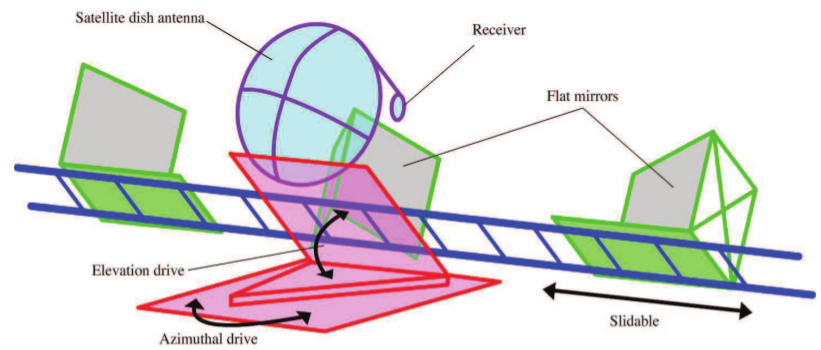
\includegraphics[scale=0.5]{figs/1.png}
\caption{Pictorial illustration of the Stony Brook's Michelson-type radio interferometer: the mirrors  can slide through the rail for adjustable baseline lengths. The Central dish stays on front of the satellite dish antenna. }
\label{2-sketch}
\end{center}
\end{figure}


\bigskip


\subsection{The Detection and Analysis Systems}\label{detection_system}

The electronic part of the experiment is composed of commercial receiver amplifier (satellite finder)  and analog-to-digital converter (labpro) connected to a computer \cite{sbu}. The output is given in voltage (volt) by time (seconds), and acquired in the computer through the software {\it LoggerPro} \cite{loggerpro}. To convert the observed spectra to {\it power response}, we use the specified {\it Voltage (V) versus Power(dBm) curve}, figure \ref{conv}, in the appendix. The slope is reported as  $s = - 25(mV/dB),$ resulting on
\begin{equation}
P_{dBm} (t)  = \frac{u(t) \mbox{ V}}{(-25 \mbox{ mV})},
\label{pdb}
\end{equation}
with the conversion of {\it decibel m} into a linear power scale is
\begin{equation}
P (t)  = 10^{\frac{P_{dBm}(t) - 30}{10}}.
\label{pdb2}
\end{equation}




\bigskip

\subsection{Methodology of the Observations}\label{observations}

After the initial calibration (subsection \ref{calibration}), we proceeded with the data acquisition, which is divided on four parts:

\begin{enumerate}
 \item {\bf Satellite's Single Dish Response}: After positioning the receiver directly the coordinates of of a point source, \eg a geostationary TV satellite, we performed two scans of the power response  for the  single dish, with $\Delta \theta^{single}_{4,5} = 10^o$, varying azimuthally.

 \item {\bf Sun's Single Dish Response}:After positioning the receiver directly to the Sun (azimuth and elevation showed in the table \ref{a-sun}), we performed three scans of its power response, with $\Delta \theta^{sin}_{1,2,3} = 15^o$, varying azimuthally. From this measurement, and normalizing with the previous satellite's measurements, we marginally infer the Sun's angular diameter, $\Phi_{sun}^{Sin}$.

 \item {\bf Sun's Interferometer Response}: The receiver is  faced to the interferometer central mirror, and, after calibration, we performed five scans of the power response of the Sun, with five different baselines lengths,  $B^{meas}_{1,2,3,4,5}$, and  with $\Delta \theta^{sun}_{1,2,3,4,5} = 20^o$.

 \item {\bf Satellite Source's Interferometer Response}: We performed five scans of the power response of the point source, with the same five different baseline lengths, $B^{meas}_{1,2,3,4,}5$, and  with $\Delta \theta^{sat}_{1,2,3,4,5} = 10^o$.
\end{enumerate}


\bigskip


\subsection{Methodology of the Calibration}\label{calibration}

The calibration of the radiotelescope was performed in the following way:
\begin{description}
 \item [Calibrating the azimuth disk and the elevation dial with Sun]  We need this to minimize the effect of the telescope aperture attenuation on the measurement of $P_{max}$ and $P_{min}$ (equation (\ref{vis})) when we measure the Sun. In another words, the central maximum of the interference pattern should be $\theta = \theta_0$ of the source. With the correct position of the Sun (table \ref{a-sun}) we point the single dish detector directly to it and, together with an analogical Satellite Finder and the LoggerPro software, we find the position with highest intensity, scanning vertically. We then trail the elevation dial to the corrected aligned. We use the latter shadow to align the sun (looking to its shadow) and the azimuth disk can be calibrated.

\item [Calibrating the Mirrors] For the {\it Interferometry} observation, we rotate the dish to the center of the central mirror, with the left and right mirror on their closest position from the center. We maximize the signal by refining the aim of the telescope. First, measuring the power for the left mirror alone. Then, performing the measurement with the right mirror alone. We verifies how the reflected intensities matches. 
\end{description}

 
\bigskip






\section{Data Reduction}
% description of how reduced and calibrated  your data

In this session we discuss how we treat the raw data, which was registered with the  software LoggerPro \cite{loggerpro} as measurements of the total output voltage vs time of  signal.

\subsection{Treatment of the Voltage V(t) Raw Data}

To normalize and delogarithm  all the four sets of data described in the section \ref{observations},  we use the equations (\ref{pdb}) and (\ref{pdb2}). The negative slope indicates that the output voltage decreases as the input power increase. The interferometry results for the Sun and for the satellite are shown in the figures \ref{voltpow2} and \ref{voltpow3}. The total power is the amplitude squared of the summed  electric vectors of the electromagnetic signals, as we described before.




 \begin{figure}[htb]
\begin{center}
 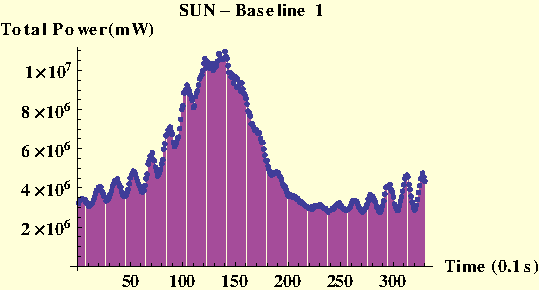
\includegraphics[scale=0.7]{plots/sun1pow.pdf}
 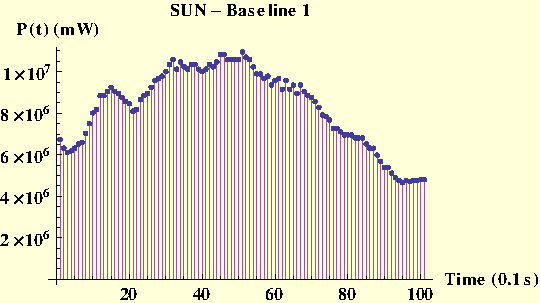
\includegraphics[scale=0.7]{plots/sun1powc.pdf}
 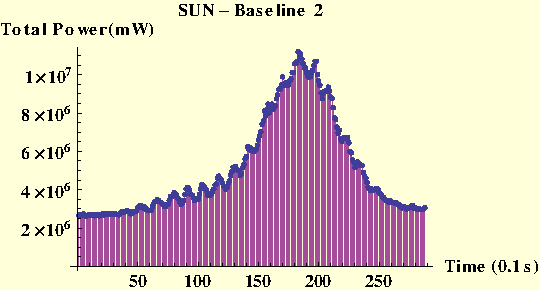
\includegraphics[scale=0.7]{plots/sun2pow.pdf}
 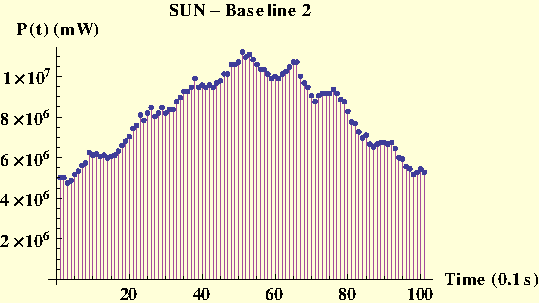
\includegraphics[scale=0.7]{plots/sun2powc.pdf}
 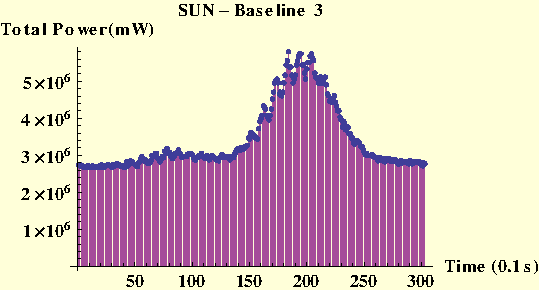
\includegraphics[scale=0.7]{plots/sun3pow.pdf}
 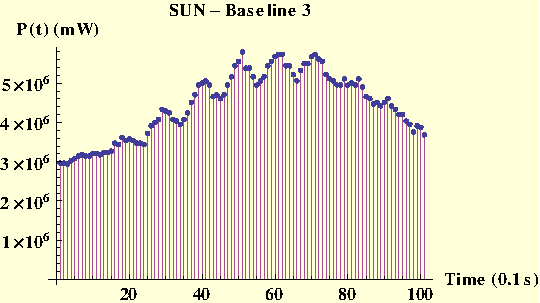
\includegraphics[scale=0.7]{plots/sun3powc.pdf}
 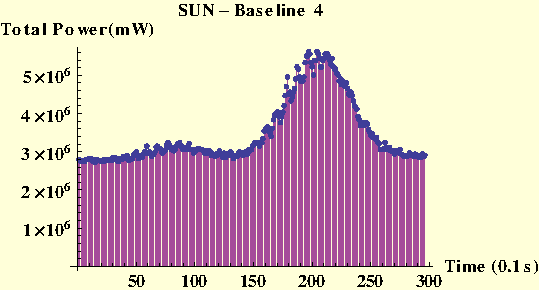
\includegraphics[scale=0.7]{plots/sun4pow.pdf}
 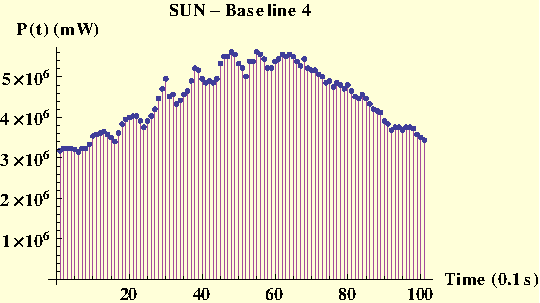
\includegraphics[scale=0.7]{plots/sun4powc.pdf}
 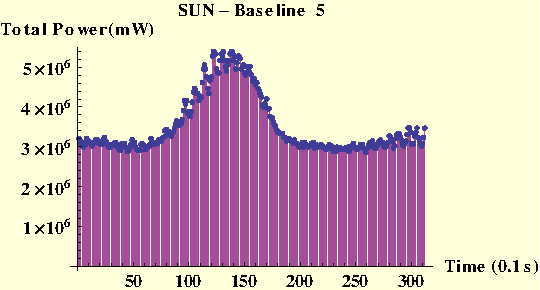
\includegraphics[scale=0.7]{plots/sun5pow.pdf}
 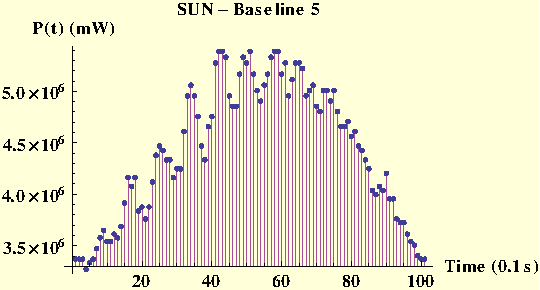
\includegraphics[scale=0.7]{plots/sun5powc.pdf}
\caption{Interferometer measurements of total power of the Sun, in function of time, for the five set of measurements. On the right, after the  cuts.}
\label{voltpow2}
\end{center}
\end{figure}

 \begin{figure}[htb]
\begin{center}
 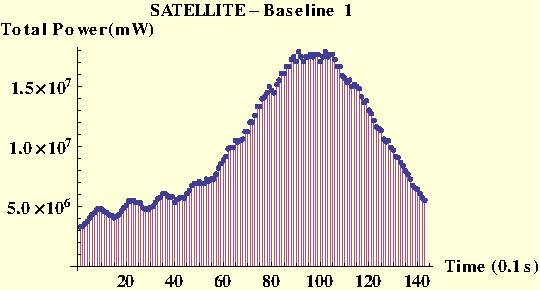
\includegraphics[scale=0.7]{plots/sat1pow.pdf}
 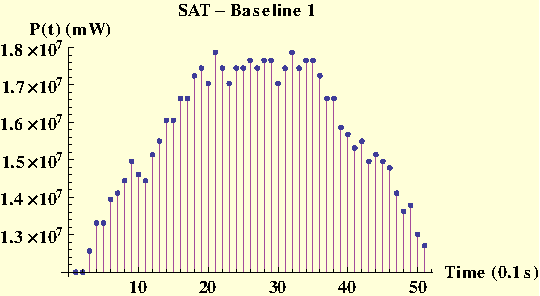
\includegraphics[scale=0.7]{plots/sat1powc.pdf}
 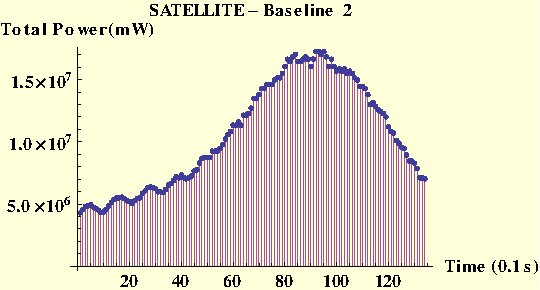
\includegraphics[scale=0.7]{plots/sat2pow.pdf}
 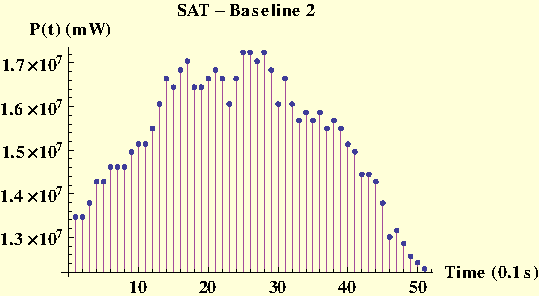
\includegraphics[scale=0.7]{plots/sat2powc.pdf}
 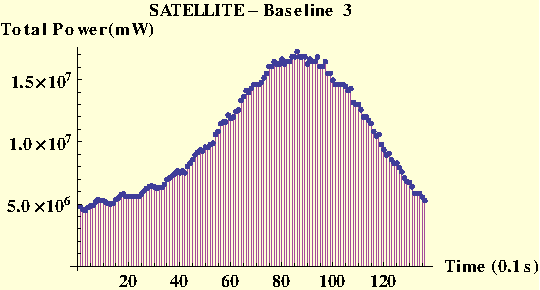
\includegraphics[scale=0.7]{plots/sat3pow.pdf}
 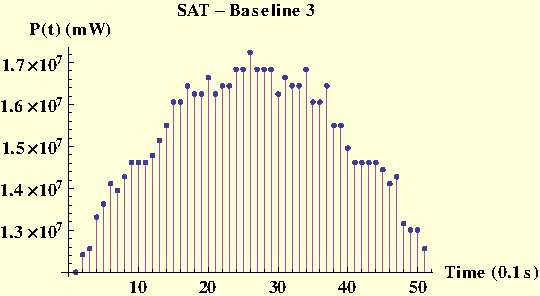
\includegraphics[scale=0.7]{plots/sat3powc.pdf}
 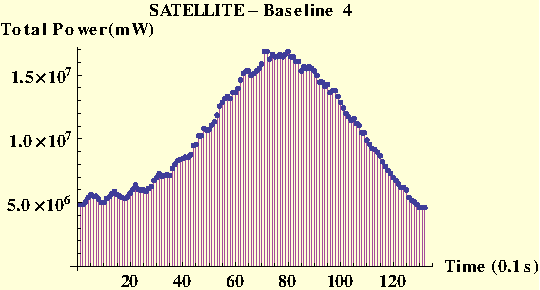
\includegraphics[scale=0.7]{plots/sat4pow.pdf}
 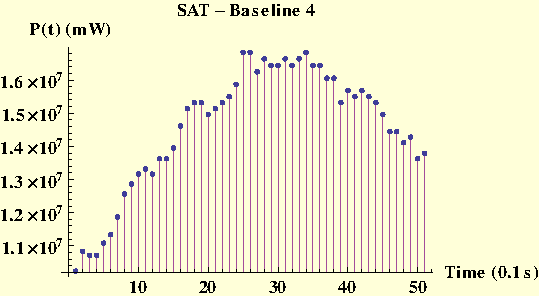
\includegraphics[scale=0.7]{plots/sat4powc.pdf}
 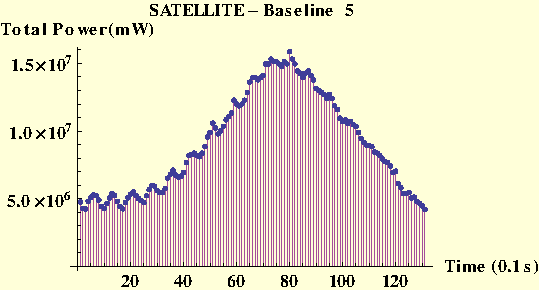
\includegraphics[scale=0.7]{plots/sat5pow.pdf}
 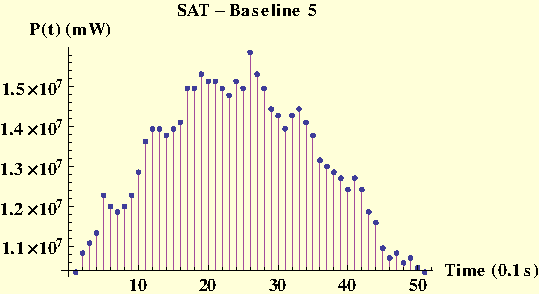
\includegraphics[scale=0.7]{plots/sat5powc.pdf}
\caption{Interferometer measurements of total power of the satellite, in function of time, for the five set of measurements. On the right, after the  cuts.}
\label{voltpow3}
\end{center}
\end{figure}




\bigskip


\subsection{The Single Dish Measurements for the Sun and the Satellite}

In the single dish mode, the size of the solar disk is the {\it deconvolution} of the single dish solar profile with the single dish satellite profile. We report the single dish profile for one of the measurements of each of the sources in the figure \ref{voltpow4}. We use these two profiles to resolve a first approximation of the solar angular diameter.

 \begin{figure}[htb]
\begin{center}
 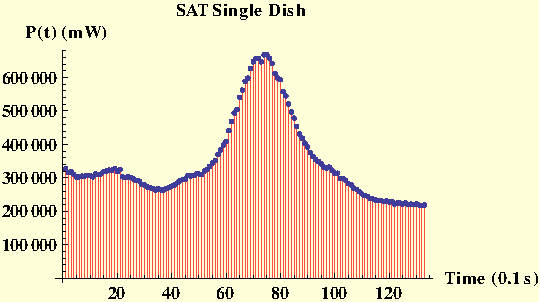
\includegraphics[scale=0.8]{plots/single/1.pdf}
 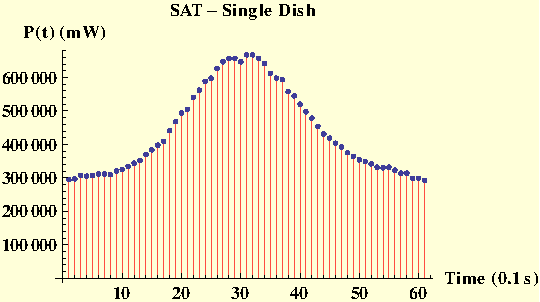
\includegraphics[scale=0.8]{plots/single/2.pdf}
 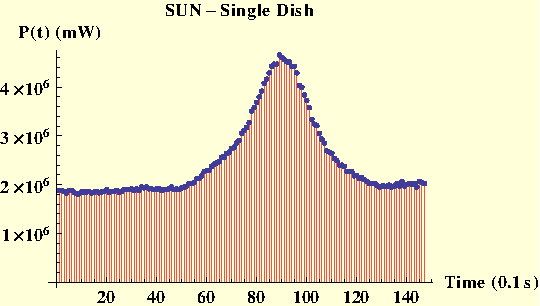
\includegraphics[scale=0.8]{plots/single/3.pdf}
 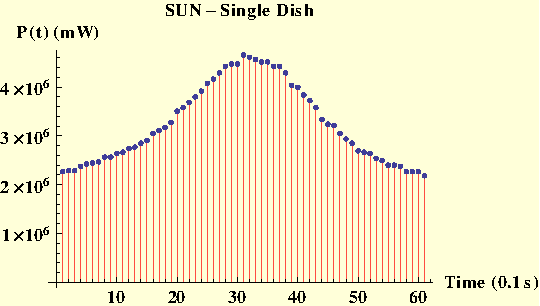
\includegraphics[scale=0.8]{plots/single/4.pdf}

\caption{Single dish measurements for the Sun and the satellite.}
\label{voltpow4}
\end{center}
\end{figure}



\section{Data Analysis and Results}
% description of any analytically steps: parameter estimation, error estimation, model-fitting...



\subsection{Single Dish's Estimation of the Sun's Angular Diameter}

We  obtain a first estimative of the angular diameter of the Sun by comparing the Fourier components of the single dish measurements of the Sun and of the satellite. The size of the solar disk is the deconvolution of the single-dish solar profile with the single-dish satellite profile,
$$FFT(\Phi_{sun}^{Sin}) = \frac{FFT^{Sin}_{sun}}{FFT^{Sin}_{sat}},$$
resulting on the figure \ref{11}. We approximate the  central peak by a normal distribution and calculate the {\it full width at half maximum} (FWHM), as rough value for the  diameter of the Sun, $\Phi^{Sin}_{sun} \approx 25' $.


 \begin{figure}[htb]
\begin{center}
 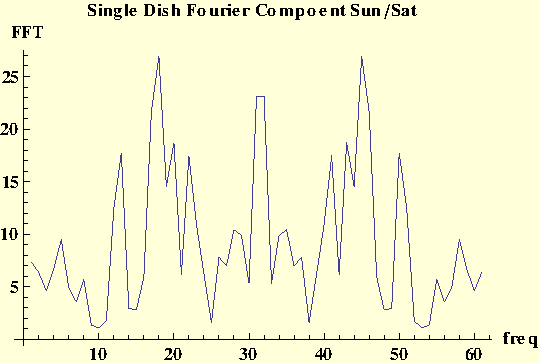
\includegraphics[scale=1.2]{plots/single.pdf}
\caption{The Sun's single dish Fourier component  over the satellite's. We  obtain a first calculation of the angular diameter of the Sun by calculating the FWHM of the central peak and Fourier transforming it. }
\label{11}
\end{center}
\end{figure}

\bigskip
\subsection{Calculation of the  Baselines  and Visibility Functions}
We calculate the baseline lengths for the set of five measurements of the Sun and of the satellite with the equation (\ref{BB}), converting the object's azimuth to the declination value, as in equation (\ref{dec}). The fringe frequency was numerically calculated by the Fourier transform profiles of the the total power data. The final values are shown in the table \ref{baselines} in the appendix.

From the same Fourier profiles we calculated the $P_{max}$ and $P_{min}$ points, as shown in the session \ref{visb}. The visibility functions are automatically obtained from the equation (\ref{vis}). 





\bigskip
\subsection{Obtaining the $\Phi_{sun}$ by Taylor-Approximating the Visibility Function} \label{taylormet}

The first method to estimate the value of the diameter of the sun is by plunging the values we have obtained for the visibility function into a Taylor approximation of the visibility equation (\ref{vissinc}),
$$ V_{sun}^{Tay}  = \frac{\sin(x)}{x} \approx \frac{x-x^3/6}{x} = 1 - \frac{x^2}{6}$$
where $x=\pi B_{\lambda} \Phi^{Tay}_{sun} $.

This gives  a value in radians for the  diameter of the Sun for one baseline, and it can later converted into arc minutes. A {\it Fast Fourier Transform} (FFT) of the fringe pattern shows a peak at the frequency of the fringe period $\Delta t$. Together with the equation (\ref{BB}), the angular diameter of the Sun can be calculated by
\begin{equation}
\Phi_{sun}^{Tay} = \frac{\sqrt{6}}{\pi} \frac{1}{B_{\lambda}} \sqrt{1 - V_{sun}^{Tay}(B_{\lambda})}.
\label{vistay}
\end{equation}

The mean and the standard deviation  for the five values obtained from this method results on $\Phi^{Tay}_{sun} = 37.43' \pm 5.33'$.



\bigskip

\subsection{Obtaining $\Phi_{sun}$ by Fitting the Fourier Components} \label{fitmet}


The second method to calculate the angular diameter of the sun is based on the fact that each measurement gives one Fourier component for baseline length. In the observations we obtain five Fourier components, $V_{sun}(B_{\lambda})$, which are a Fourier transformation of the energy density distribution, $\varepsilon(\theta_0)$. 

Plotting   $V_{sun}(B_{\lambda})$ vs. $B_{\lambda}$  exhibits  the Fourier transformation of the object structure. Since the structure of the Sun should be a {\it top-hat function}, the resulting plot (for its Fourier transformation) is exactly the {\it sinc function},
$$V^{fit}_{sun}(B_{\lambda}) = \mbox{ sinc }(B_{\lambda} {\Phi^{fit}_{sun}}),$$
 we saw in the equation (\ref{vissinc}). The sinc function sinc(x), also called the {\it sampling function} and  arises frequently in signal processing and the theory of Fourier transforms \cite{wiki}. 

We plot the Fourier components of the visibility function versus their baseline lengths, shown in the figure \ref{sing}. The fit gives the value of  $\Phi^{Fit}_{sun}= 32.77' \pm 5.28'$.




 \begin{figure}[htb]
\begin{center}
 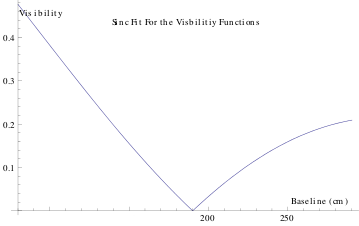
\includegraphics[scale=0.85]{plots/sinc3.png}
 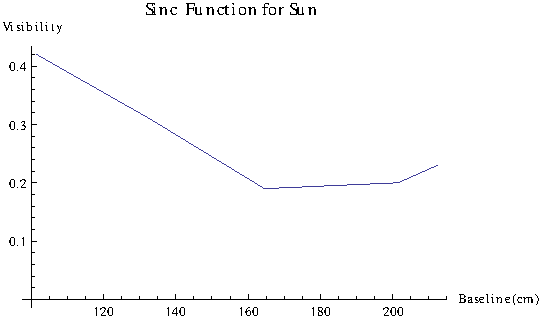
\includegraphics[scale=0.85]{plots/sinc1.pdf}
\caption{The Fourier components of the visibility function versus baselines, which is fitted by a sinc function, giving the value of the angular diameter of the sun. }
\label{sing}
\end{center}
\end{figure}



\bigskip
\subsection{Chi-Squared Fitting}
We use our knowledge of the {\it variance} (the measure of how far a set of numbers is spread out) of the measurements to fit it statistically by using the weighted sum of squared errors:
$$X^2 = \sum_i \frac{(O_i-E_i)^2}{\sigma_i^2}.$$

We assume that the variances, $\sigma^i$,  or our measurements are Gaussian functions and the the above equation will follow a {\it chi-squared distribution}. We obtain $\chi^2 = 12.3$ for the previous analysis.

\section{Discussion} % contextual interpretation of your results and a comparison with established results and practices; a discussion of why you may not be seeing the expected result, and so possible changes or improvement to your data taking
 
There were many source of errors in this experiment due to incorrect calibration and positioning of the sources. The most relevant source of uncertainties, was the  incorrect alignment of the  two side mirrors. Due to this fact we see that our profiles are not clean, most of the times not having a clean central peak. 

Despite the high uncertainties, the calculations surprisingly resulted on a good agreement to the expect value for the diameter of sun in the literature. The second method, based on the fit of the Fourier components, resulted on a more precise value, as it was expect. It is not clear how better theses results can be when treating very accurate and calibrated data instead.
\section{Conclusion}
% recapitulation of results and what we learned


Performing two complementary analysis: (i) the Taylor expansion of the visibility function, and (ii) the fitting of the visibility function, we have found  two values for the angular diameter of the sun, respectively,  $\Phi^{Tay}_{sun} = 37.43' \pm 5.33' $ and $\Phi^{Fit}_{sun}= 32.77' \pm 5.28'$. These results are compatibles between themselves and to the value registered in the literature,  $\Phi^{Actual}_{sun}= 31.1' \pm 0.6'$ \cite{wiki}. 

From the present results we  conclude that despite the simple character of the radio interferometer utilized in this experiment, it shown to be qualified to perform radio interference at radio wavelengths.


%%%%%%%%%%%%%%%%%%%%%%%%%%%%%%%%%%%%%%%%%%%%%%%%%%%%%%

\begin{thebibliography}{2}

\bibitem{michel} (1) Albert A. Michelson, Francis G. Pease, {\it Measurement of the diameter of alpha Orionis with the interferometer}, Astrophys. J. 53, 249-259 (1921).
\bibitem {sbu} (2) J. Koda \& J. Barret, {\it Stony Brook Radio Interferometer}, 2012.
\bibitem {wiki} (3) \url{http://www.wikipedia.org/} as 03/01/2012.
\bibitem {brand} (4) H. Bradt, {\it Astronomy Methods}, Cambridge University Press, 2007.
\bibitem{jackson} (5) J. D. Jackson, {\it Classical Electrodynamics}, (Third Edition), 1998. 


\bibitem[Dishpointer (2012)] {satbb} (6) Satellite Finder, \url{http://www.dishpointer.com/}, February/2012.
\bibitem[Navy (2012)] {sunbb} (7) Sun Altitude/Azimuth Table, \url{http://aa.usno.navy.mil/data/docs/AltAz.php}, February/2012.
\bibitem{loggerpro} (8)\url{ http://www.vernier.com/products/software/lp}.

\bibitem{math} (10) \url{ http://www.wolfram.com/mathematica/}.
\bibitem{root} (9) \url{http://root.cern.ch/drupal/}.
\end{thebibliography}

\clearpage


\appendix



\begin{deluxetable}{ccrrrrrrrrcrl}
\tabletypesize{\scriptsize}

\tablecaption{Elevation and Azimuth of the Sun for 02/26/2012 \cite{sunbb}}
\tablewidth{0pt}
\tablehead{
\colhead{Eastern Time } & \colhead{Elevation} & \colhead{Azimuth (E of N)} 
}
\startdata                                                                                 
10:50 &      37.4   &    155.2\\
11:00  &     38.1   &    159.3\\
11:10   &    38.7   &    162.3\\
11:20   &    39.2   &    165.4\\
11:30 &      39.7   &    168.6\\
11:40  &     40.0   &    171.8\\
11:50   &    40.2   &    175.0\\
12:00   &    40.3   &    178.2\\
12:10   &    40.3    &   181.5\\
12:20  &     40.2    &   184.7\\
\enddata
\tablecomments{The altitude and azimuth of the Sun for the day of the observations, 02/26/2012,  at Stony Brook University, NY,W 73 08, N40 56.}
\label{a-sun}
\end{deluxetable}


\begin{deluxetable}{ccrrrrrrrrcrl}
\tabletypesize{\scriptsize}

\tablecaption{Measured and Calculated Baseline Lengths }
\tablewidth{0pt}
\tablehead{
\colhead{Baseline Measured  } & \colhead{Length (m)} & \colhead{Baseline Satellite } & \colhead{ Length (m)} & \colhead{Baseline Sun }& \colhead{Length (m)}}
\startdata                                                                                 
$B^{meas}_{1}$ & $0.60 \pm 0.05$ & $B^{sat}_{1}$& $1.40 \pm 1.16$ & $B^{sun}_{1}$  & $1.01 \pm 1.16$\\
$B^{meas}_{2}$ & $0.76 \pm 0.05 $ & $B^{sat}_{2}$& $1.62 \pm 1.16$ & $B^{sun}_{2}$ & $1.33 \pm 1.16$\\
$B^{meas}_{3}$ & $0.92 \pm 0.05$& $B^{sat}_{3}$& $1.85 \pm 1.16$ & $B^{sun}_{3}$ & $1.64 \pm 1.16$\\
$B^{meas}_{4}$&  $1.08 \pm 0.05$ & $B^{sat}_{4}$& $2.16 \pm 1.16$ & $B^{sun}_{4}$ & $2.02 \pm 1.16$\\
$B^{meas}_{5}$ & $1.24 \pm  0.05$ &$B^{sat}_{5}$& $2.30 \pm 1.16$  & $B^{sun}_{5}$ & $2.13 \pm 1.16$ \\
\enddata
\tablecomments{The first values are the baseline lengths  measured from the left border of the left mirror to the right border of the right mirror. The accurate length measurement should have be done from the middle of the both mirror. In the final calculations we use the baseline lengths calculated from the analysis, \ie the second and third values of the table. The measured  values are included for completeness only.  Although the uncertainty for them (which are based on the half of the minimum size of the ruler) are smaller than for the calculated values, it does not imply that the first values are more precise.}
\label{baselines}
\end{deluxetable}





\begin{deluxetable}{ccrrrrrrrrcrl}
\tabletypesize{\scriptsize}

\tablecaption{Time and Angle Range for the Interferometer Measurements for the Sun}
\tablewidth{0pt}
\tablehead{
\colhead{Baseline Label in the Analysis } & \colhead{Filename} & \colhead{Angle Range  in Degrees} & \colhead{Eastern Time} & \colhead{Sun's Azimuth}}
\startdata                                                                                 
$B^{sun}_{1}$ &  SUN1&-10,10 &1050&155.2\\
$B^{sun}_{2}$&	SUN2 &-15,5&1105&	162.3\\
$B^{sun}_{3}$&	SUN3&	-15,5&1115	&165\\
$B^{sun}_{4}$&	SUN41&	-15,5&1118	&165.4\\
$B^{sun}_{4}$&	SUN42&	-10,10	&1120	&165.4\\
$B^{sun}_{5}$&	SUN5&	-10,10	&1123	&165.4\\
\enddata
\tablecomments{Data from the log book. The file SUN42 is the same data than SUN41 so it was not used in the analysis. We refer to SUN4 instead than SUN41.}
\label{sun}
\end{deluxetable}


\begin{deluxetable}{ccrrrrrrrrcrl}
\tabletypesize{\scriptsize}

\tablecaption{Time and Angle Range for the Interferometer Measurements for the Satellite}
\tablewidth{0pt}
\tablehead{
\colhead{Baseline Label in the Analysis } & \colhead{Filename} & \colhead{Angle Range in Degrees} & \colhead{Eastern Time} & \colhead{Satellite's Azimuth}}
\startdata   
$B^{sun}_{1}$& SAT1	&	20,30	&	1219  & \\
$B^{sun}_{2}$& SAT2	&	20,30	&	1217
 &  \\
$B^{sun}_{3}$& SAT3	&	20,30	&	1215
 & \\
$B^{sun}_{4}$& 	SAT4	&	20,20	&	1213
 &   \\
$B^{sun}_{5}$& SAT5	&	20,30	&	1205
&   \\
\enddata
\tablecomments{Data from the log book.}
\label{sat}
\end{deluxetable}


 \begin{figure}[htb]
\begin{center}
 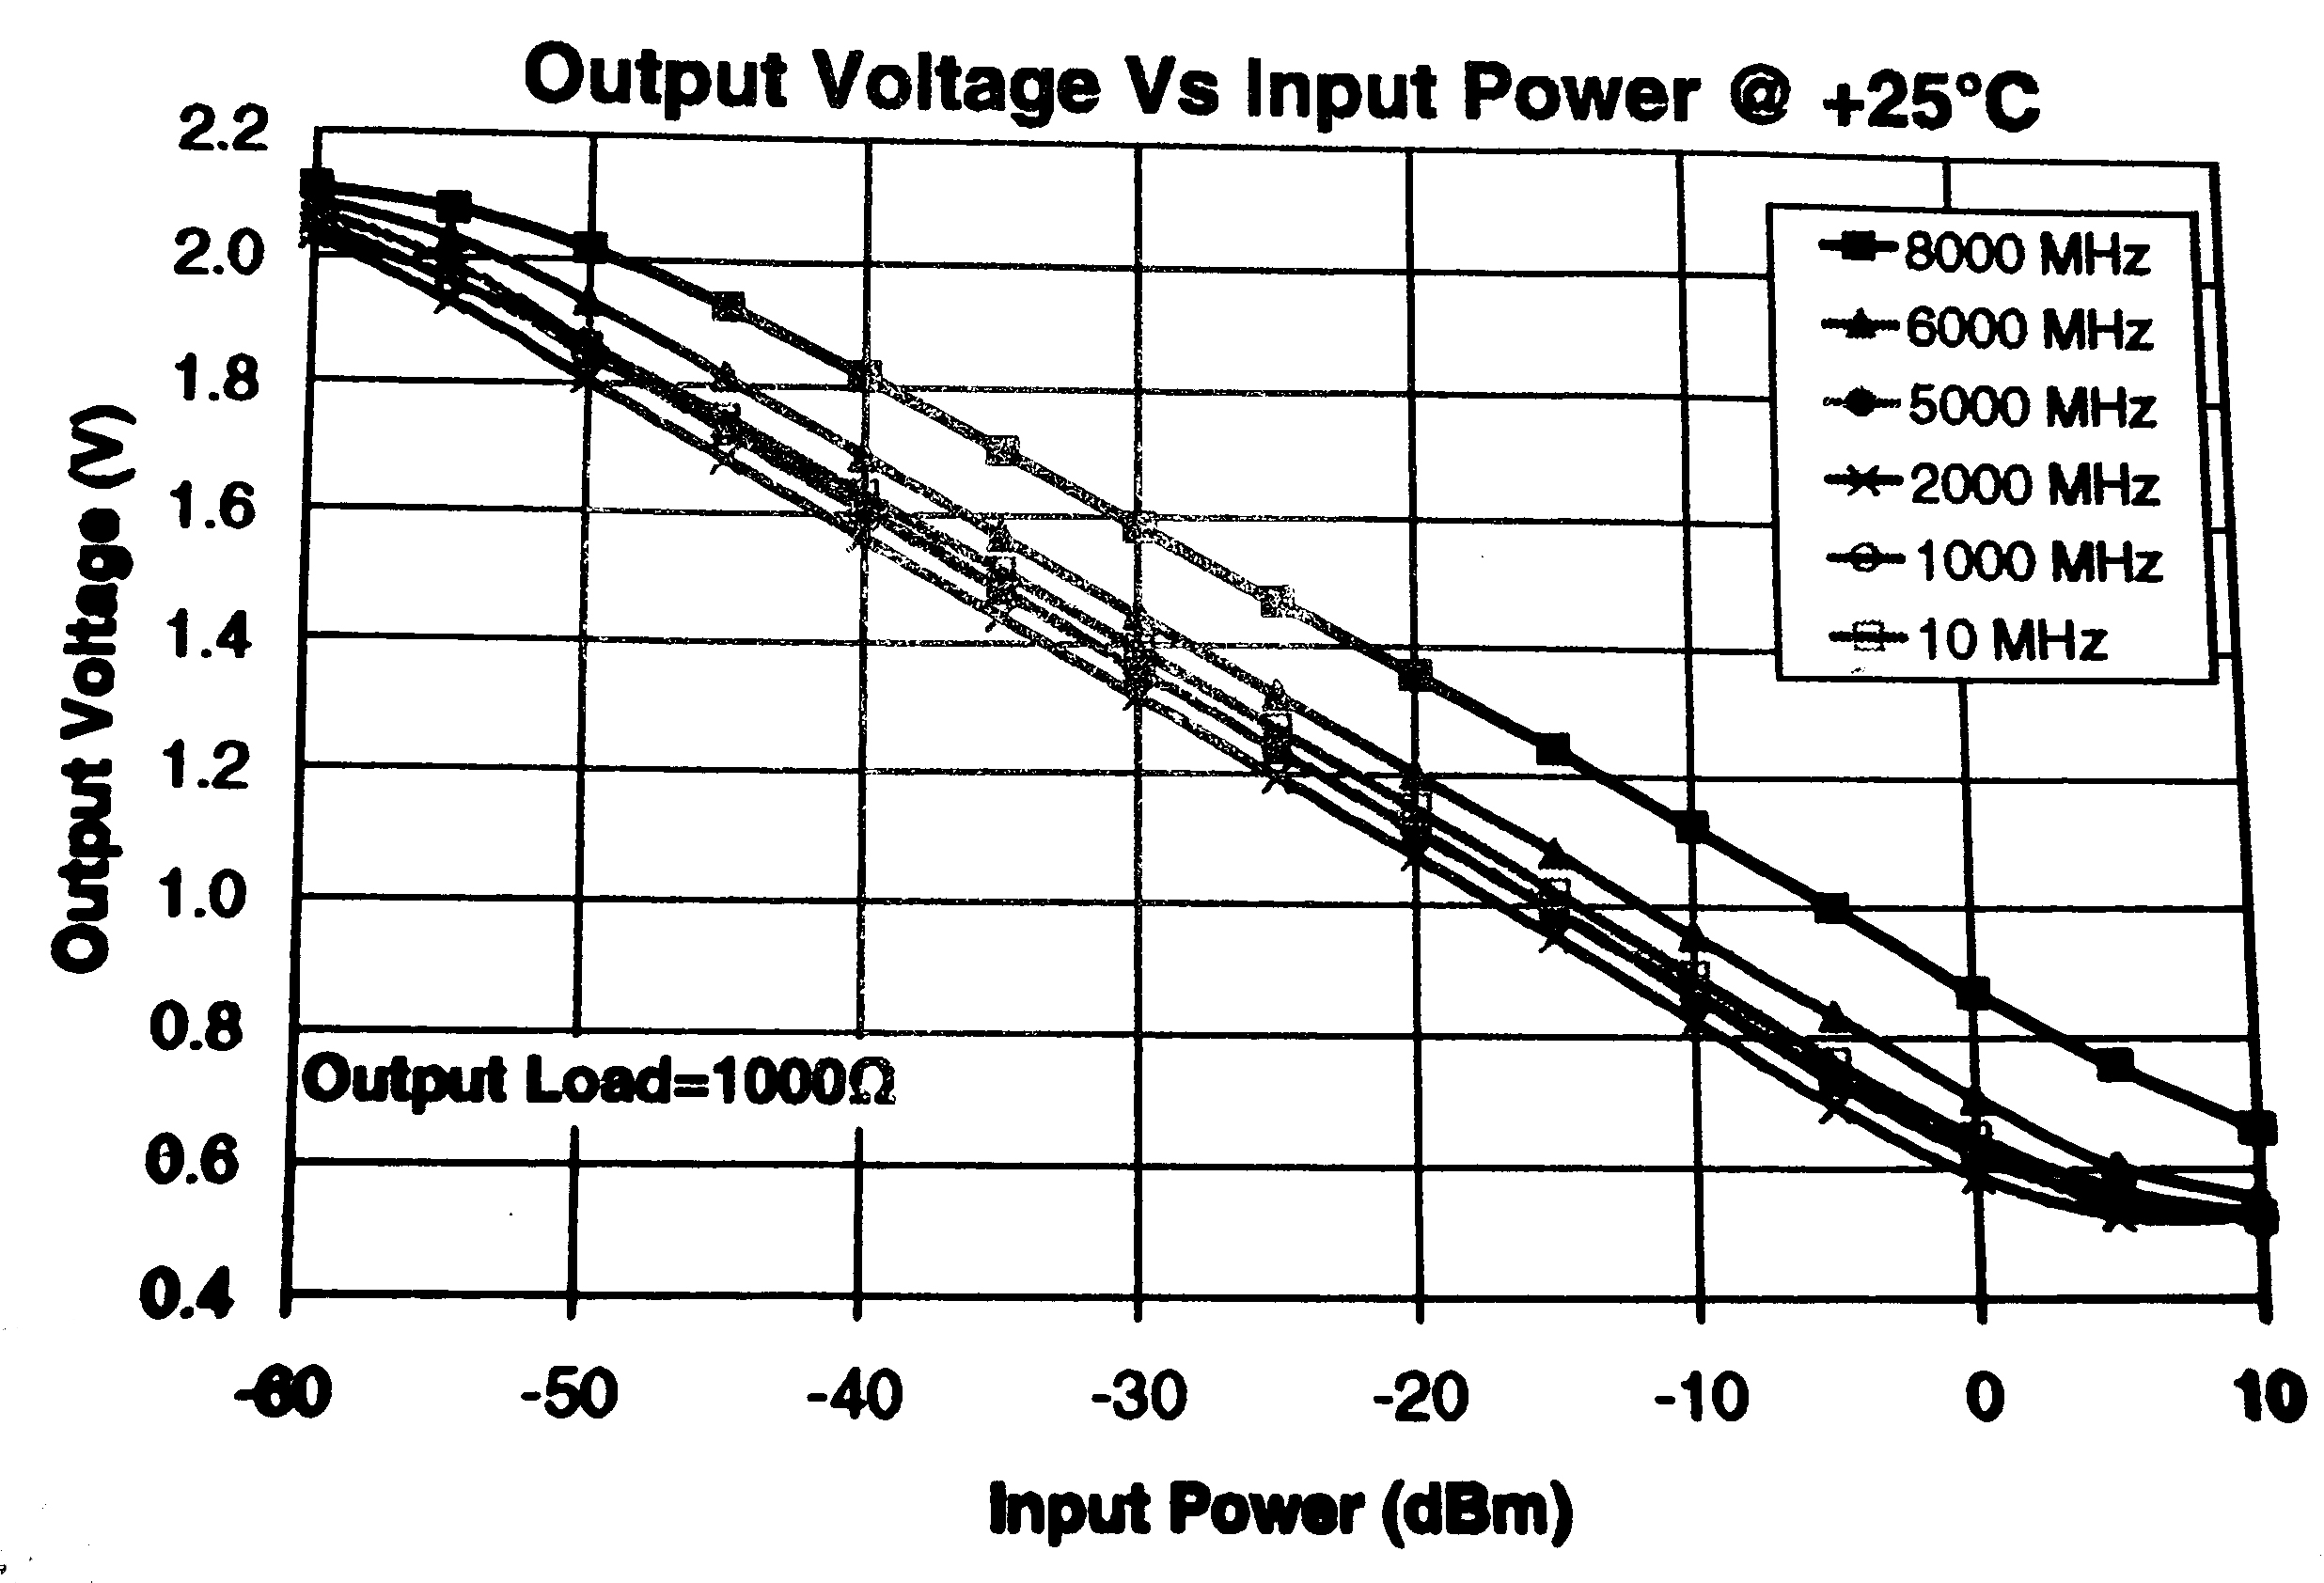
\includegraphics[scale=0.15]{figs/voltage_curve.JPG}
\caption{The convertor from voltage to power. }
\label{conv}
\end{center}
\end{figure}

 \begin{figure}[htb]
\begin{center}
 \includegraphics[scale=0.5]{code/errors.png}
\end{center}
\end{figure}

\end{document}
